\documentclass{swfubeamer}

\RequirePackage{ctex} % fontspec loaded here
%\ctexset{today=old}

\usepackage{pifont}
\usepackage{biolinum}
\newcommand\Ctrl[1]{\LKeyCtrlX{#1}} % for Ctrl-u Ctrl-l

\begin{document}
\begin{frame}
  \title{基于Linux的操作系统研究}
  \author{杨鑫}
  \titlepage
  \vfill
  \tiny{
    \ding{70} 计算机科学与技术\\
    \ding{41} cynyang777@gmail.com\\
    \ding{37} 13099930449
  }
\end{frame}
%\frame{\titlepage}

\begin{frame}{操作系统组成模块}
  \begin{itemize}
  \item 启动模块
  \item 进程模块
  \item 内存模块
  \item 外围功能模块
  \end{itemize}
\end{frame}

\begin{frame}{开发环境}
  \begin{itemize}
  \item<1-4> 宿主OS
  \item<2-4> 虚拟机
  \item<3-4> 编译器
  \item<4-4> 编缉器
  \end{itemize}
  \begin{tabular}[center]{|l|c|}\hline
  \uncover<1-4> {\textit{debian}} & \uncover<1-4> {Linux debian v6.1.0.7-amd64}\\
  \uncover<2-4> {\textit{bochs}}  & \uncover<2-4> {Bochs v2.6.9}\\
  \uncover<3-4> {\bf nasm}        & \uncover<3-4> {Nasm v2.16.01}\\
  \uncover<3-4> {\bf gcc}         & \uncover<3-4> {Gcc v12.2.0}\\
  \uncover<4-4> {\textit{Emacs}}  & \uncover<4-4> {\small{GNU Emacs v28.2}}\\
  \uncover<4-4> {\textit{Vim}}  & \uncover<4-4> {\small{GNU Vim v0.7.2}}\\\hline
  \end{tabular}
\end{frame}

\begin{frame}{启动过程}
  \begin{center}
    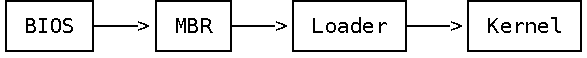
\includegraphics[width=.7\linewidth]{boot}
  \end{center}
\end{frame}

\begin{frame}{shell}
  \begin{itemize}
     \item 清屏\Ctrl{L};
     \item 清除输入\Ctrl{U};
    \end{itemize}
  \begin{center}
    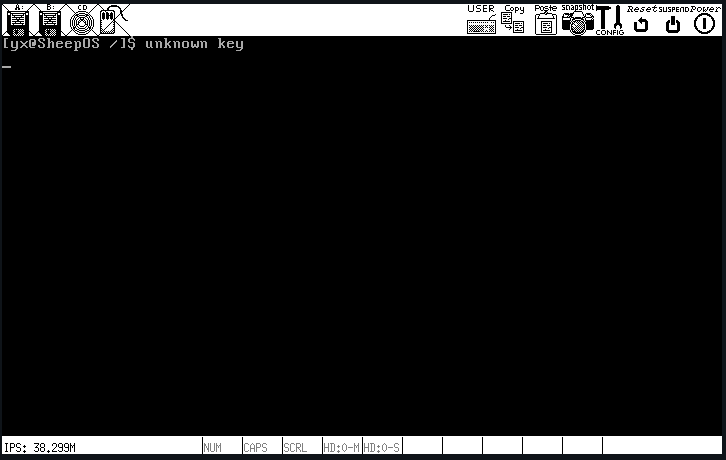
\includegraphics[width=.7\linewidth]{shell}
  \end{center}
\end{frame}

\begin{frame}{查看目录——ls}
  \begin{center}
    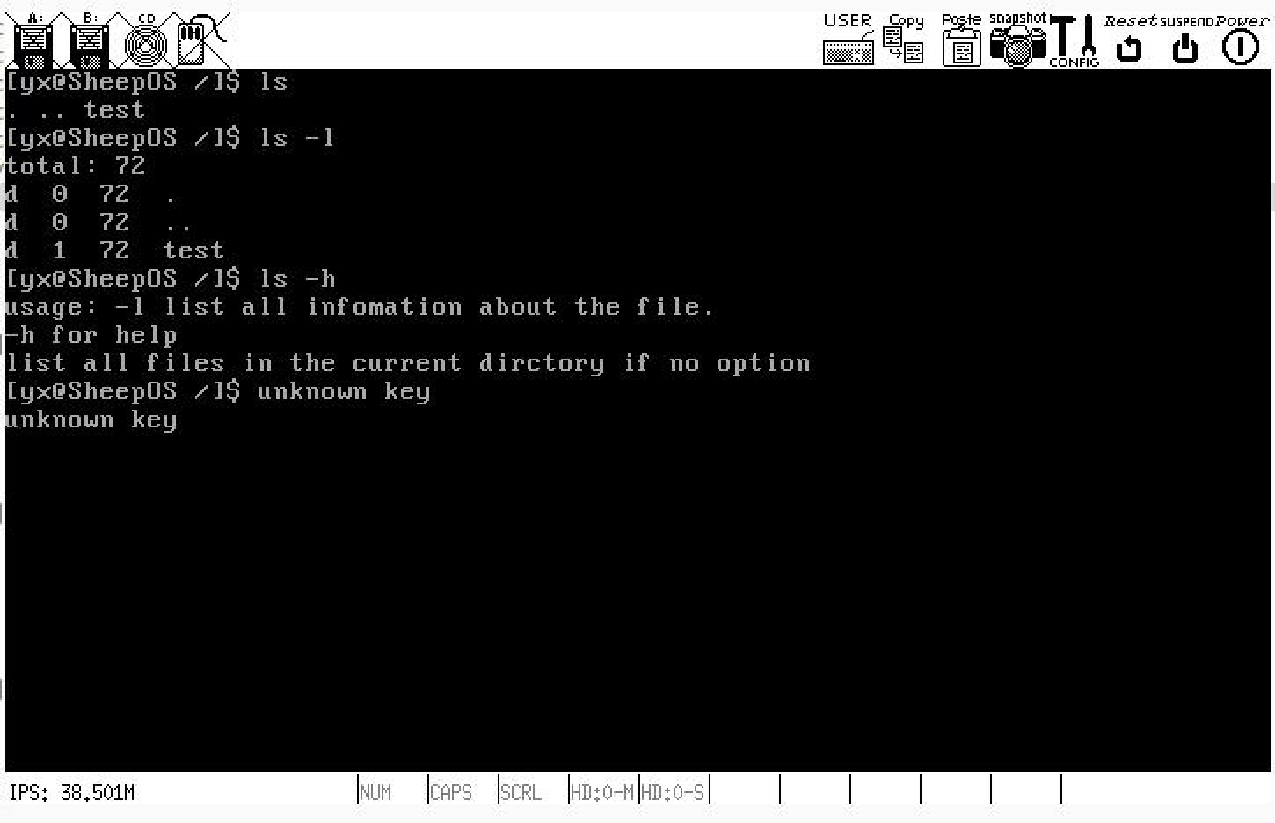
\includegraphics[width=.8\linewidth]{ls}
  \end{center}
\end{frame}

\begin{frame}{跳转到指定目录——cd}
  \begin{center}
    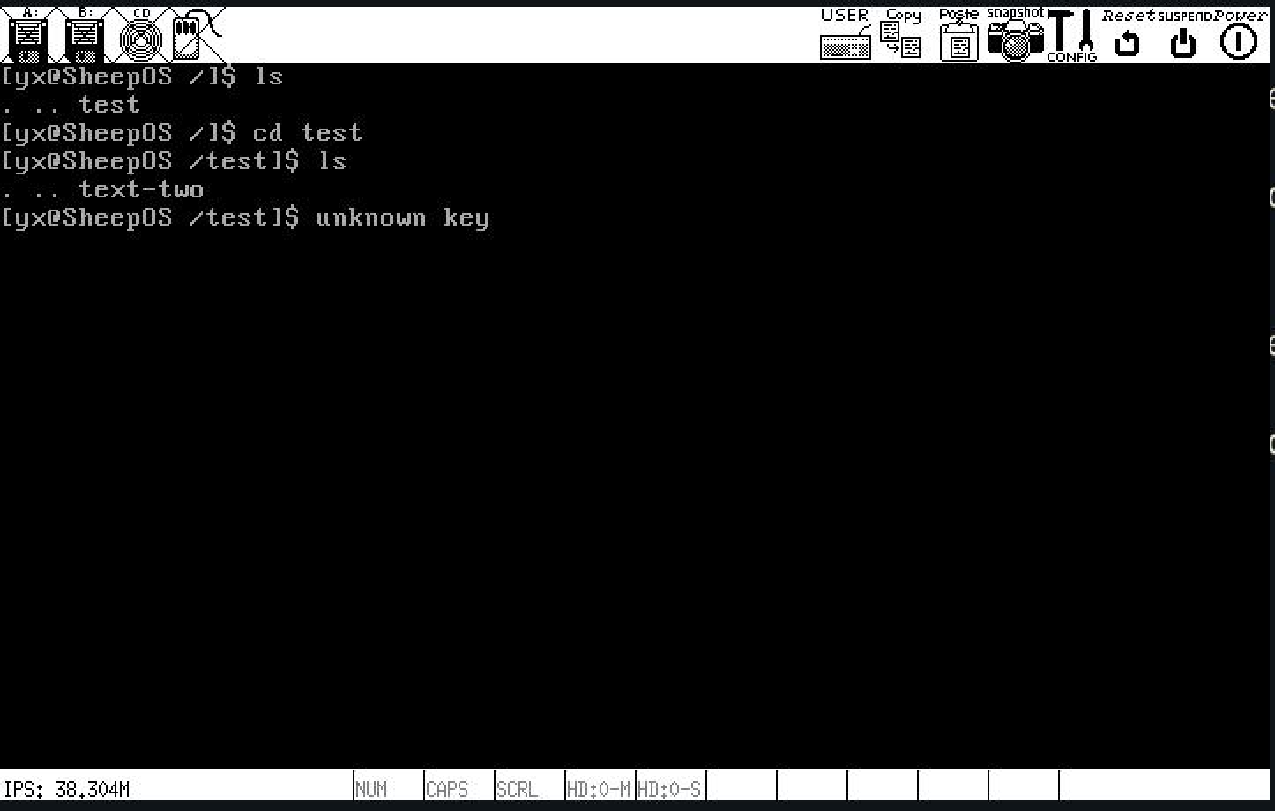
\includegraphics[width=.8\linewidth]{cd}
  \end{center}
\end{frame}

\begin{frame}{创建文件——mkdir}
  \begin{center}
    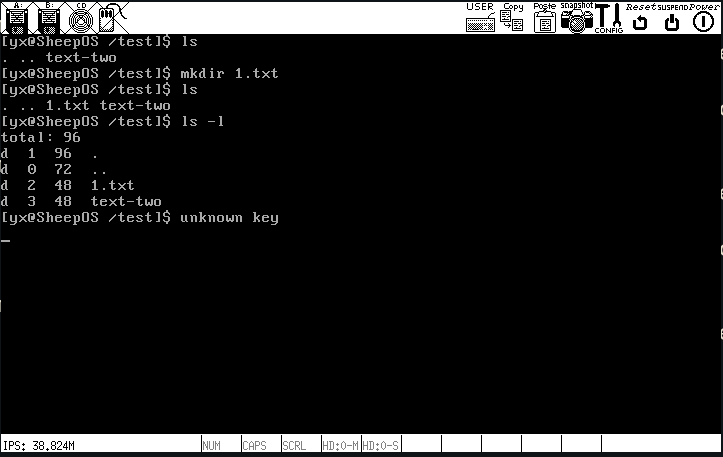
\includegraphics[width=.8\linewidth]{mkdir}
  \end{center}
\end{frame}

\begin{frame}{删除文件——rmdir}
  \begin{center}
    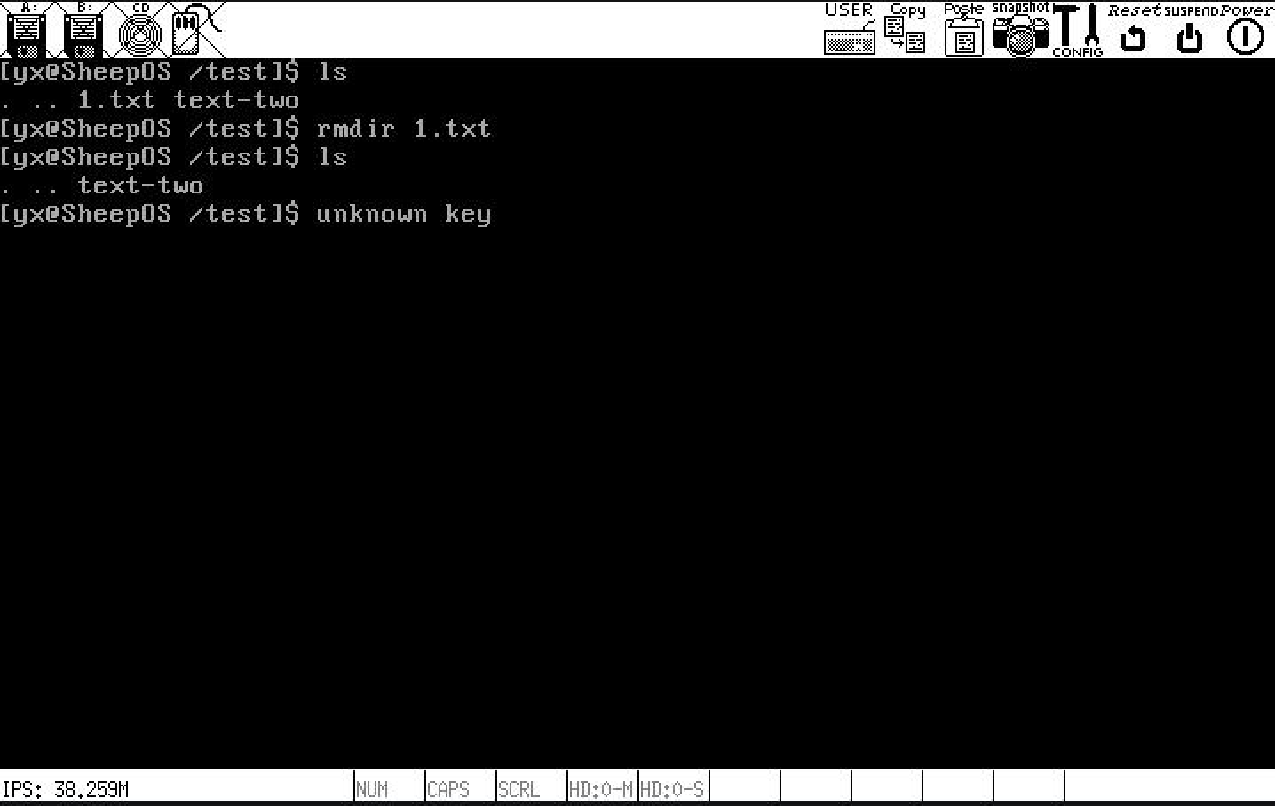
\includegraphics[width=.8\linewidth]{rmdir}
  \end{center}
\end{frame}

\end{document}


%%% Local Variables:
%%% mode: latex
%%% TeX-master: t
%%% TeX-master: t
%%% TeX-master: t
%%% TeX-master: t
%%% End: